\chapter{Probabilistic Method}
\section{Dominating Set}

\textbf{The Problem}
Given a graph:
\[
G=(V,E)
\]
find a smallest possible subset:
\[
D\subseteq V
\]
such that every vertex in the graph is either:
\begin{itemize}
    \item contained in \(D\), or
    \item adjacent to some vertex in \(D\).
\end{itemize}

Such a set is called a \emph{dominating set}.

Intuitively, we may think of the vertices in \(D\) as ``control centers'' or ``facilities'' such that every location in the graph is either itself a facility or directly connected to one.

Unfortunately, finding the minimum dominating set is NP-hard, so we want to find a polynomial time algorithm that gives us a 
reasonably small\footnote{We care more about the asymptotic behaviour of the size of set produced by the algorithm and less about which polynomial time complexity the algorithm has.} dominating set.
\subsection*{A Randomised Solution}

Suppose the graph has minimum degree \(d\). We now consider the following extremely simple randomised strategy:

\begin{quote}
Choose \(k\) vertices randomly out of the n vertices (uniformly among the $\binom{n}{k}$ possible choices).
If the chosen set forms a dominating set, output it. Otherwise, try again!
\end{quote}
At first glance, this algorithm seems dumb. 
However, it turns out that if we choose \(k\) large enough, the probability of failure becomes small.
The key question thus becomes:
\begin{quote}
What is the probability of failure as a function of \(k\), \(n\), and \(d\)?
\end{quote}
We now analyse this probability.

\subsection*{Probability That a Vertex Remains Undominated}

Fix a vertex $v\in V$. Since the graph has minimum degree \(d\), $N[v]$ contains 
at least $d+1$ vertices. For \(v\) to remain undominated, none of the selected \(k\) 
vertices may lie inside $N[v]$

When choosing vertices uniformly at random, the probability that a single chosen vertex does \emph{not} belong to \(N[v]\) is at most:
\[
1-\frac{d+1}{n}
\]

\[
\implies
\Pr[v\text{ remains undominated}]
\le
\left(1-\frac{d+1}{n}\right)^k
\]

Using the inequality\footnote{Refer \autoref{exp_inequality}} $1-x\le e^{-x}$ for all $x\in\mathbb{R}$, we obtain:
\[
\Pr[v\text{ remains undominated}]
\le
e^{-k(d+1)/n}
\]

\subsection*{Bounding the Failure Probability}

The algorithm fails if at least one vertex remains undominated.

Applying the union bound\footnote{Refer \autoref{union_bound}}

\[
\Pr[\text{failure}]
\le
n\cdot e^{-k(d+1)/n}
\]

We would like this probability to be strictly less than \(1\). Therefore we require:
\[
n e^{-k(d+1)/n}<1
\]

\[
\implies
\ln n-\frac{k(d+1)}{n}<0
\]

\[
\implies
k>\frac{n\ln n}{d+1}
\]

Thus, choosing:
\[
k=\frac{cn\ln n}{d+1}
\]
for any constant $c>1$ gives 
$
\Pr[\text{failure}]
\le
n^{1-c}
$ which tends to \(0\) as \(n\to\infty\).

\subsection*{What Does This Actually Mean?}

The important point is not merely that the algorithm succeeds with high probability.

Rather, we have shown something stronger --

\begin{quote}
There exists a dominating set\footnote{
This method has a limitation - if $d<c\ln n$, 
then the size of the dominating set produced by the algorithm is basically the whole set of vertices, making it useless.} of size roughly:
\[
\frac{n\log n}{d}
\]
\end{quote}

Indeed, if no such dominating set existed, our algorithm could never possibly succeed.

Thus a simple probabilistic argument simultaneously:
\begin{itemize}
    \item proves the existence of a reasonably small dominating set,
    \item and gives a randomised algorithm capable of finding one.
\end{itemize}

\subsection*{Amplifying the Success Probability}

Even if a single run fails, we may simply repeat the algorithm independently.

If the failure probability of one run is $\bm{p}=\frac{1}{n^{c-1}}$, 
then after $\bm{t}$ independent repetitions, the probability that \emph{every} run fails equals $\bm{p^t}$
which decreases exponentially fast. \\

So the tradeoff is choosing a larger $c$ has a smaller expected number of repetitions ($\frac{n^{c-1}}{n^{c-1}-1}$)\footnote{Since the probability of failure is $p=(n^{c-1}-1)/n^{c-1}$ and this is a bernoulli trial, the expected number of trials for success is 1/p } but a larger dominating set,
while choosing a smaller $c$ has a larger expected number of repetitions but a smaller dominating set.

\section{Bipartite Subgraph}

\textbf{Problem statement.}
Given an undirected graph $G=(V,E)$ with $|E|=m$, we wish to find a bipartition of $V$ that maximizes the number of edges between vertices of different partitions.
Equivalently, we want a 2-coloring of the vertices that maximizes the number of bichromatic edges. We aim to show that we can always guarantee at least $m/2$ edges in the cut.

\subsection{Expected Number of Bichromatic Edges}
Let X be the number of bichromatic edges under a random 2-coloring of the vertices. 
Each edge has a probability $\frac{1}{2}$ of being bichromatic, so define the indicator variable $I_{i}$ as 1
 when the edge numbered $i$ is bichromatic and 0 otherwise. We can conclude that for a random vertex 2-coloring, 
 Pr($I_{i}=1$)=$\frac{1}{2}$ and Pr($I_{i}=0$)=$\frac{1}{2}$, so $\mathbb{E}[I_{i}]=\frac{1}{2}$.
Since $X=\sum_{i=1}^{m}I_{i}$, we have:
\[
\mathbb{E}[X]=\mathbb{E}[\sum_{i=1}^{m}I_{i}]=\sum_{i=1}^{m}\mathbb{E}[I_{i}]=\frac{m}{2}
\]

\subsection*{A Weak Lower Bound}

Let $X\in\{0,1,\dots,m\}$ be the number of bichromatic edges under a random 2-coloring of the vertices. We already have
$\mathbb{E}[X]=\frac{m}{2}$. \\

\noindent We derive a crude lower bound on $\Pr\!\left(X\ge \frac{m}{2}\right)$.

\medskip
\noindent\textbf{Case 1: $m=2k$ (even).}\\

\noindent Let $p=\Pr(X\ge k)$. The maximum value of $E(X)$ under these constraints would be achieved 
when we push all mass in $\{0,1,\dots,k-1\}$ to $k-1$, and all mass in $\{k,\dots,2k\}$ to $2k$. Then
\[
\mathbb{E}[X]\le (1-p)(k-1)+p(2k).
\]

Using $\mathbb{E}[X]=k$,
\[
k \le (1-p)(k-1)+2kp
\]
\[
k \le k-1+p(k+1)
\]
\[
1 \le p(k+1)
\]
\[
p \ge \frac{1}{k+1}=\frac{2}{m+2}.
\]

\[
\implies
\Pr\!\left(X\ge \frac{m}{2}\right)\ge \frac{2}{m+2}.
\]

\medskip
\noindent\textbf{Case 2: $m=2k+1$ (odd).}\\

\noindent Let $p=\Pr(X\ge k+1)$. The maximum value of $E(X)$ under these constraints would be achieved when
all mass in $\{0,1,\dots,k\}$ is pushed to $k$, and all mass in $\{k+1,\dots,2k+1\}$ is pushed to $2k+1$. 
Then
\[
\mathbb{E}[X]\le (1-p)k+p(2k+1).
\]

Using $\mathbb{E}[X]=k+\tfrac{1}{2}$,
\[
k+\frac{1}{2} \le k+p(k+1)
\]
\[
\frac{1}{2} \le p(k+1)
\]
\[
p \ge \frac{1}{2(k+1)}=\frac{1}{m+1}.
\]

\[
\implies
\Pr\!\left(X\ge \frac{m}{2}\right)\ge \frac{1}{m+1}.
\]

\medskip
\textbf{Conclusion --}
\[
\Pr\!\left(X\ge \frac{m}{2}\right)\ge min(\frac{2}{m+2},\frac{1}{m+1}) = \frac{1}{m+1}.
\]

\subsection{A Simple Randomised Algorithm}

From the probabilistic analysis, a random coloring satisfies
\[
\Pr\left(X \ge \frac{m}{2}\right) \ge \frac{1}{m+1}.
\]

Therefore, if we repeatedly sample random colorings independently, 
the probability that none of $T$ trials succeeds is at most
\[
(1-\frac{1}{m+1})^T.
\]

\noindent Choosing $T=(m+1)\ln(m+1)$ gives
\[
(1-\frac{1}{m+1})^T
\le
e^{-\frac{T}{m+1}}
=
e^{-\ln(m+1)}
=
\frac{1}{m+1}
\]
Which goes to 0 as $m\to\infty$.

While simple, this method does not exploit structure of intermediate solutions and relies purely on repeated random sampling rather than improvement steps.

\subsection{Derandomisation}

Instead of making random choices, we assign vertices one by one 
smartly, trying to maximise the number of bichromatic edges.
Suppose some vertices have already been assigned and the remaining vertices are
still unassigned. Let X be the random variable denoting the number of bichromatic edges.
Let L and R be the bipartitions.\\


Denote the expected value of X given the first \(i\) assignments by:
\[
\mathbb E[X \mid i]
\]


For the $i+1$-th assignment of vertex \(v\), we have two choices:
\begin{itemize}
\item place \(v\) in \(L\),
\item place \(v\) in \(R\).
\end{itemize}

The current conditional expectation is the average of the expectations obtained
from these two choices. Therefore, at least one choice must yield a conditional
expectation that is at least as large as the current one.

\[
\max \left( \mathbb E[X \mid \text{i, v in L}], \mathbb E[X \mid \text{i, v in R}] \right) >= \frac{1}{2} \left(\mathbb E[X \mid \text{i, v in L}] + \mathbb E[X \mid \text{i, v in R}] \right) = \mathbb E[X \mid i]
\]


We simply assign the next vertex such that it would add the most 
bichromatic edges in this step -- that choice yields a better expectation for the future.
\vspace{0.5em}

\[
\text{Since I have ensured that }\mathbb E[X \mid i+1] \ge \mathbb E[X \mid i]
\]

\[
\implies \mathbb E[X \mid \text{n assignments}] \ge \mathbb E[X \mid \text{0 assignments}]
\]

\[
\implies X_{final} \ge \frac{m}{2}
\]

\vspace{0.5em}

\noindent\textbf{Why did that work?}\\


\noindent Initially $\mathbb E[X]=\frac{m}{2}$. At every step we choose an 
assignment that does not decrease the conditional
expectation\footnote{This is by no means a proof for optimality -- it does not 
maximise the number of bichromatic edges.}. Hence the conditional expectation never drops below \(m/2\)!\\


\noindent After all vertices have been assigned, no randomness remains. The conditional
expectation is then equal\footnote{If you are feeling tricked somehow, 
I relate fully! But it is true, we designed this deterministic algorithm and simultaneously proved that 
it produces at least \(m/2\) crossing edges using conditional expectation!} to the 
actual number of crossing edges produced by the algorithm.

\[
\implies
X_{final} \ge \frac{m}{2}.
\]

\noindent Thus we obtain a deterministic algorithm that always constructs a bipartite
subgraph containing at least half of the edges.\\


\noindent\textbf{Why does this not work for all problems?}\\


\noindent The properties of this particular problem we needed for this to work were -- 

\noindent \begin{enumerate}
\item $E[X \mid 1] = m/2$, regardless of which assignment that was -- symmetry between the left and right sides.
\item It was obvious which assignment would maximise $E[X \mid i+1]$ given $E[X \mid i]$.
\end{enumerate}

\noindent Both these properties do not hold, for example, in the Dominating Set problem. Depending 
on your first choice (to put in the dominating set or dominated set), you might get a 
very good dominating set in expectation or a very bad one. An extreme counter example is a star shaped\footnote{A star shaped graph is a graph with 
one central node and \(n-1\) nodes connected to it and only it.} 
graph, where if you put the central node in dominated set you will get a dominating set of size \(n-1\), 
but if you put it in dominating set you will get a dominating set of size 1. 
The second property also fails because in further choices it is not 
clear how to choose which set to put the node in to maximise the conditional expectation.


\section{Array Construction}

\subsection*{The Problem}

In this problem, we must construct an array of $4n$ integers in which each of the values
$1,2,\dots,n$ appears exactly four times, subject to the following condition --
for a value $x$, let $p_{x,1}<p_{x,2}<p_{x,3}<p_{x,4}$ be the positions of its
four occurrences. Then for every $x$ the three consecutive gaps
\[
  g_1 = p_{x,2}-p_{x,1},\qquad
  g_2 = p_{x,3}-p_{x,2},\qquad
  g_3 = p_{x,4}-p_{x,3}
\]
must be pairwise distinct. For instance, with $n=3$ the array
$[1,1,2,1,2,3,1,3,2,2,3,3]$ works because the gaps are $(1,2,3)$ for $1$, $(2,4,1)$ for $2$
and $(2,3,1)$ for $3$, each consisting of three different numbers.

\subsection*{The Solution}
Consider the naive randomised algorithm of simply generating a random array of $4n$ integers which have 4 of each 
of $\{1,2,3,\dots,n\}$. We can then check if the condition holds for each of the $n$ values and if not, 
generate again. This is a simple Las Vegas algorithm but as we will see, pretty effective 
in generating the required construction quickly.

\subsection*{Success Probability}
Let the four positions of $x$, in increasing order, be
$a_1<a_2<a_3<a_4$, and define the gaps
\[
  g_1=a_2-a_1,\qquad g_2=a_3-a_2,\qquad g_3=a_4-a_3,
\]
each a positive integer, with span $s=g_1+g_2+g_3=a_4-a_1$. Once the gaps are 
fixed, the subset is determined by the starting position $a_1$ alone, which
must satisfy $a_1\ge 1$ and $a_1+s=a_4\le N$.\\

\noindent There are therefore exactly
$N-s$ admissible subsets for each tuple of gaps with $s\le N-1$. Also note that the probability of 
two gaps being equal is the same regardless of which pair of gaps we are referring to (by symmetry).

\[
  \Pr(g_1=g_2)=\Pr(g_2=g_3)=\Pr(g_1=g_3)
\]

\subsubsection*{Two Equal Gaps}
When $g_1=g_2=g$ and $g_3=h$, $s=2g+h$. So the number of such subsets are $N-(2g+h)$. Double 
summation over all possible $g$ and $h$ will yield all valid subsets and thus the exact probability.

\[
  \Pr(g_1=g_2)
  =
  \frac{1}{\binom{4n}{4}}\sum_{g=1}^{2n-1}\left(\sum_{h=1}^{4n-2g-1}\bigl(4n-2g-h\bigr)\right)
  =
  \frac{1}{\binom{4n}{4}}\sum_{g=1}^{2n-1}\binom{4n-2g}{2}
  =
  \frac{n(2n-1)(8n-5)}{3\cdot\binom{4n}{4}}
\]

\vspace{1em}
\[
\implies
\Pr(g_1=g_2)
=
\frac{n(2n-1)(8n-5)}{n(2n-1)(4n-1)(4n-3)}
=
\frac{8n-5}{(4n-1)(4n-3)}
\approx 
\frac{1}{2n} + \Theta(\frac{1}{n^2})
\]

\subsubsection*{All Equal Gaps}
Here $g_1=g_2=g_3=g$, so $s=3g$ and the number of subsets is $4n-3g$.\\

\noindent The summation over g will go from 1 to $G=\bigl\lfloor\tfrac{4n-1}{3}\bigr\rfloor$.

\[
  \sum_{g=1}^{G}(4n-3g)
  =4nG-\frac{3G(G+1)}{2}
  =\frac{G\,(8n-3G-3)}{2}
\]

\[
\implies
  \Pr(g_1=g_2=g_3)
  =\frac{G\,(8n-3G-3)}{2\binom{4n}{4}}
  =\frac{3\,G\,(8n-3G-3)}{(2n)(2n-1)(4n-1)(4n-3)}
\]

\vspace{1em}
\noindent Taking large n approximations and $G \approx \frac{4n}{3}$ gives

\[
\Pr(g_1=g_2=g_3) \approx \frac{4n\,(8n-4n)}{(2n)(2n)(4n)(4n)} \approx \frac{1}{4n^2}
\]

\subsubsection*{Inclusion-Exclusion}

\[
  \Pr(\text{bad value})=\Pr((g_1=g_2) \;\cup\; (g_2=g_3) \;\cup\; (g_1=g_3)) 
\]

\[
  =
  \Pr(g_1=g_2)+\Pr(g_2=g_3)+\Pr(g_1=g_3)-3\cdot\Pr(g_1=g_2=g_3)+\Pr(g_1=g_2=g_3)
\]

\[
  =
  3\Pr(g_1=g_2)-2\cdot\Pr(g_1=g_2=g_3)
  \approx
  3 \cdot (\frac{1}{2n}) - 2 \cdot (\frac{1}{4n^2}) + \Theta(\frac{1}{n^2})
  \approx 
  \frac{3}{2n}
\]


\[
	\implies
	\Pr[\text{bad value}] \approx \frac{3}{2n}
\]

\subsubsection*{Overall Success Probability}
The arrangement fails exactly when the gaps of at least one value is bad. The union bound gives 
$n \cdot \frac{3}{2n} = \frac{3}{2}$ as the upper bound on overall failure which is useless. 
To find anything useful, we need to know something about how they are dependent on each other. We will skip 
the exact analysis of this interdependence and notice that the placement of one value affects the gaps of 
other value by at most 4. Since this won't affect most arrangements, they are almost\footnote{Yes, this is an 
approximation but the graph of empirical data should convince you how good it is.} independent.

\[
  \Pr[\text{success}] \approx (1-\Pr(\text{bad value}))^n \approx \left(1-\frac{3}{2n}\right)^{n}
\]

\begin{figure}[ht]
  \captionsetup{labelformat=empty}
  \centering
  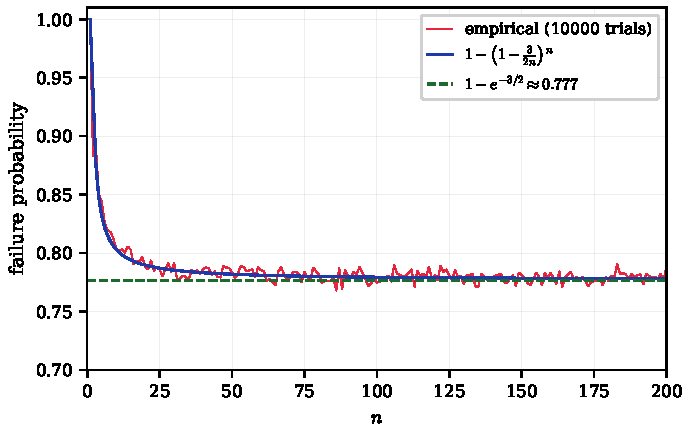
\includegraphics[width=0.78\linewidth]{../Images/randcheck_failprob.pdf}
  \caption{Interestingly, the method used to generate this graph is also a randomised algorithm -- the method of sampling. 
We used the idea of law of large numbers by saying that the number of failures divided by total number of 
runs (10000) should be a good approximation to the failure probability. Of course, 10000 was chosen 
because it was large as compared to the $n$ under consideration.}
  \label{fig:randcheck}
\end{figure}

Since each run takes $\Theta(n)$ time (generation and verification), the overall runtime 
is also expected $\Theta(n)$ using Wald's equation\footnote{Refer \autoref{wald_eq}} since we have 
expected number of runs to be $1/\Pr[\text{success}]$ which is constant hence $\Theta(1)$.

